\chapter[Solução]{solução}
  Este capítulo tem como objetivo discutir a solução utilizada durante o
desenvolvimento, assim como os resultados obtidos durante a realização do mesmo. Dentre estes
resultados, estão presentes as fontes de erros levantadas com a experiência do desenvolvimento,
suas respectivas correções, dentro do possível, e a análise da viabilidade da utilização do
sistema no contexto da reabilitação motora. Desse modo, este
capítulo está dividido nas seções: \ref{sol:solucao}, \ref{sol:fontesErro} e \ref{sol:viabilidade}.

\section{Solução}\label{sol:solucao}
  Nesta seção serão apresentadas as features envolvidas na solução do sistema,
além das ferramentas usadas. Esta será dividida em Funcionalidades -\textit{features}(\ref{sub:solFeatures}) e
ferramentas(\ref{sub:solFerramentas}).

\subsection{Funcionalidades - \textit{features}}\label{sub:solFeatures}
  As \textit{features} no desenvolvimento ágil é um pedaço de funcionalidade que oferece valor comercial \cite{versionOne}.
Geralmente as \textit{features} tem uma granularidade maior que as \textit{User Stories}(Histórias de usuário~\ref{historias}).
Podemos dizer que algumas features são compostas de \textit{User Stories}.

  O sistema possui três features, gravação de movimento, leitura de arquivo do movimento desejado e análise da repetição do movimento:
\begin{enumerate}
  \item \textbf{Gravar movimento:} Essa funcionalidade permite a gravação do movimento, deve ser feito pelo profissional fisioterapeuta
  para uma correta execução. Será esse movimento que o sistema usará como gabarito. O sistema retorna um arquivo csv.
  \item \textbf{Ler arquivo de movimento:} Essa funcionalidade espera um arquivo csv e armazena o movimento no sistema.
  \item \textbf{Praticar movimento:} Essa funcionalidade mostra a correta execução do movimento e analisa com o movimento do paciente.
\end{enumerate}

\subsection{Ferramentas}\label{sub:solFerramentas}
  Para o desenvolvimento do sistema foram usadas diversas ferramentas, a seguir serão apresentadas junto
dos artefatos gerados.
\subsection{Diagrama de sequência}\label{sub:diagramaSequencia}
  Consiste em um diagrama que tem o objetivo de mostrar como as mensagens entre os objetos são trocadas no decorrer do tempo para a realização de uma operação.\cite{diagramaSequencia}
Como pode ser visto em \ref{diagramaFisio} e \ref{diagramaPaciente}, existe dois momentos de trocas de mensagens, uma com o usuário como fisioterapeuta e outra
com o paciente.

\begin{figure}[!h]
\centering
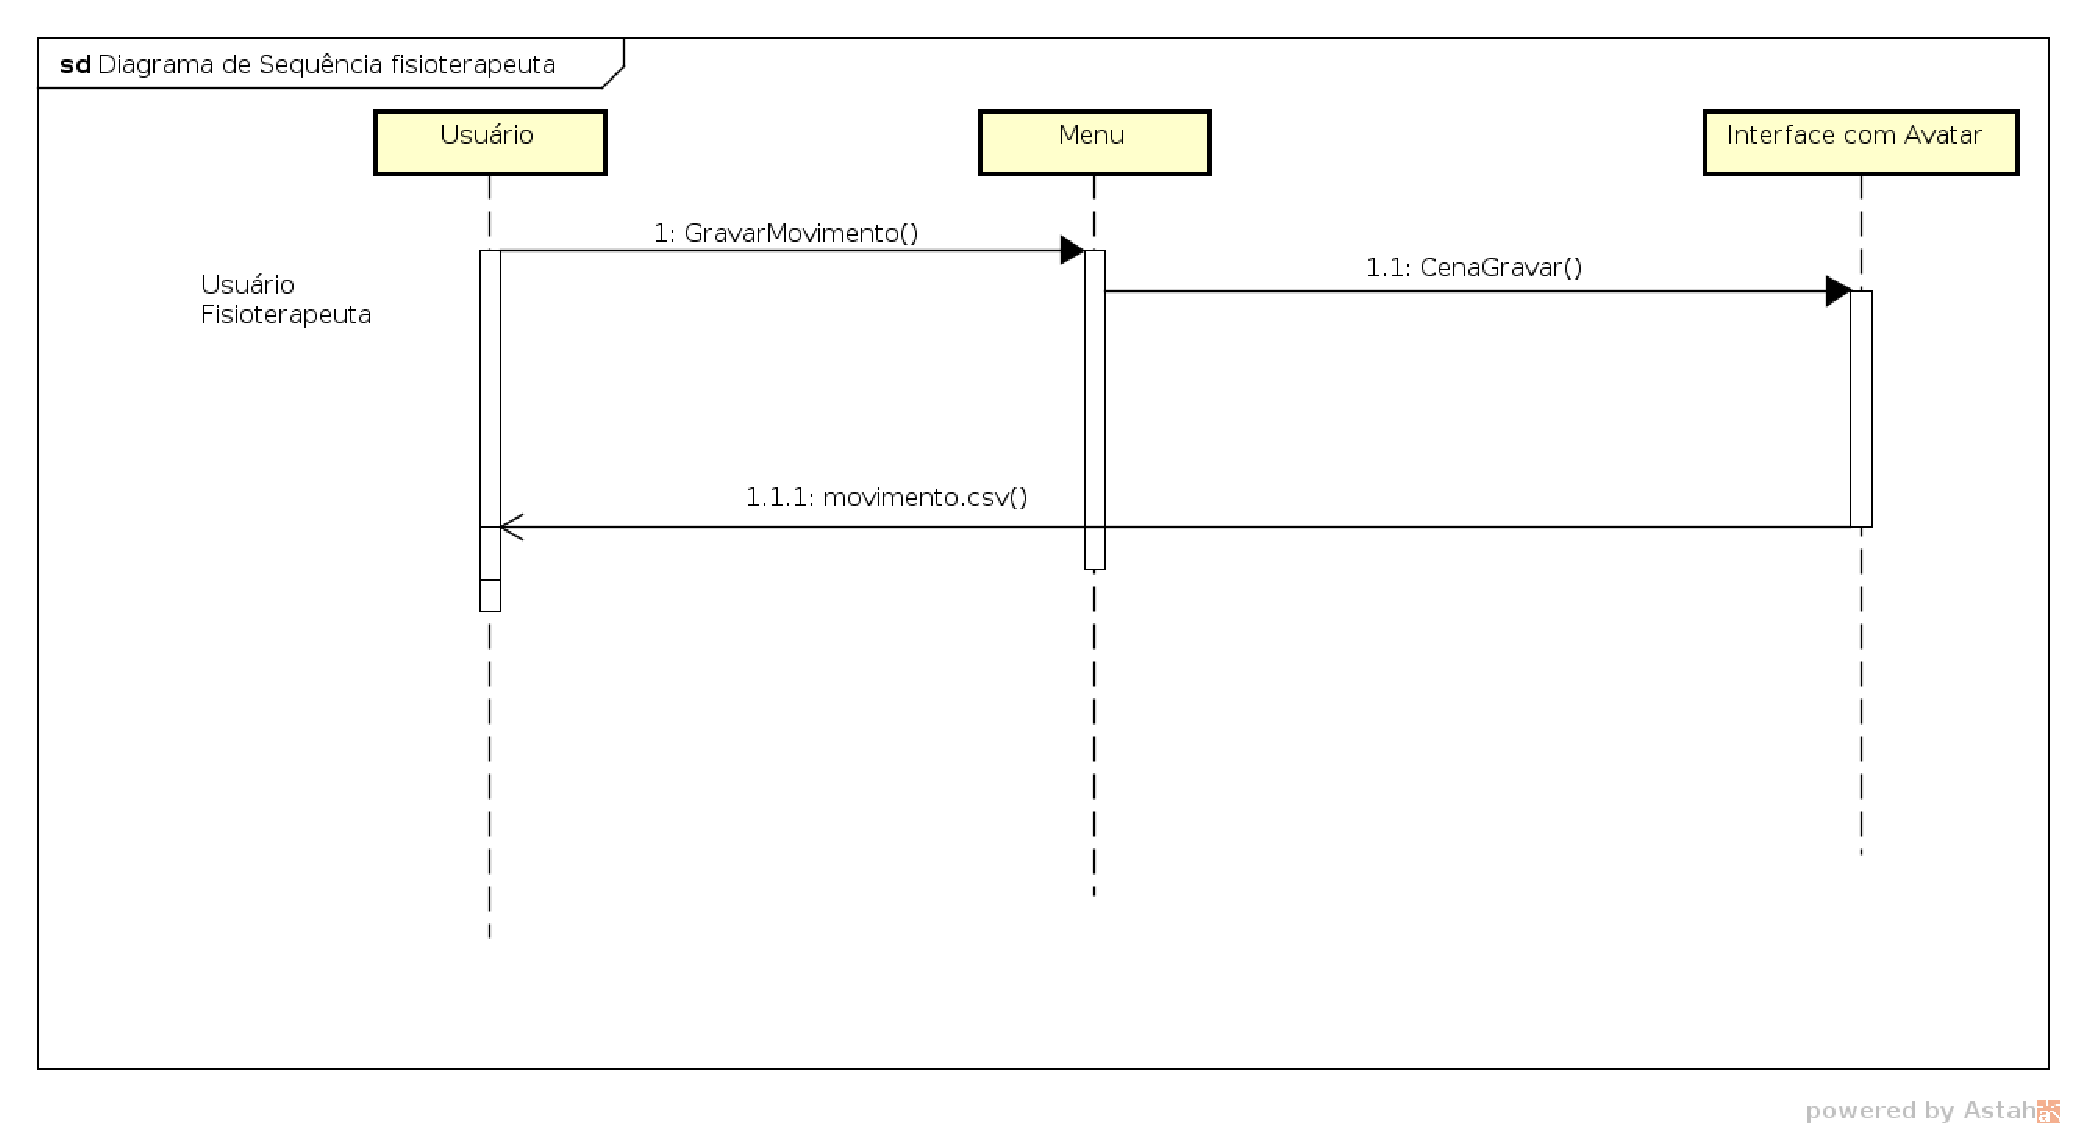
\includegraphics [keepaspectratio=true,scale=0.45]{figuras/diagramaFisio.eps}

\caption{Diagrama de sequência referente ao uso do fisioterapeuta}
\label{diagramaFisio}
\end{figure}

\begin{figure}[!h]
\centering
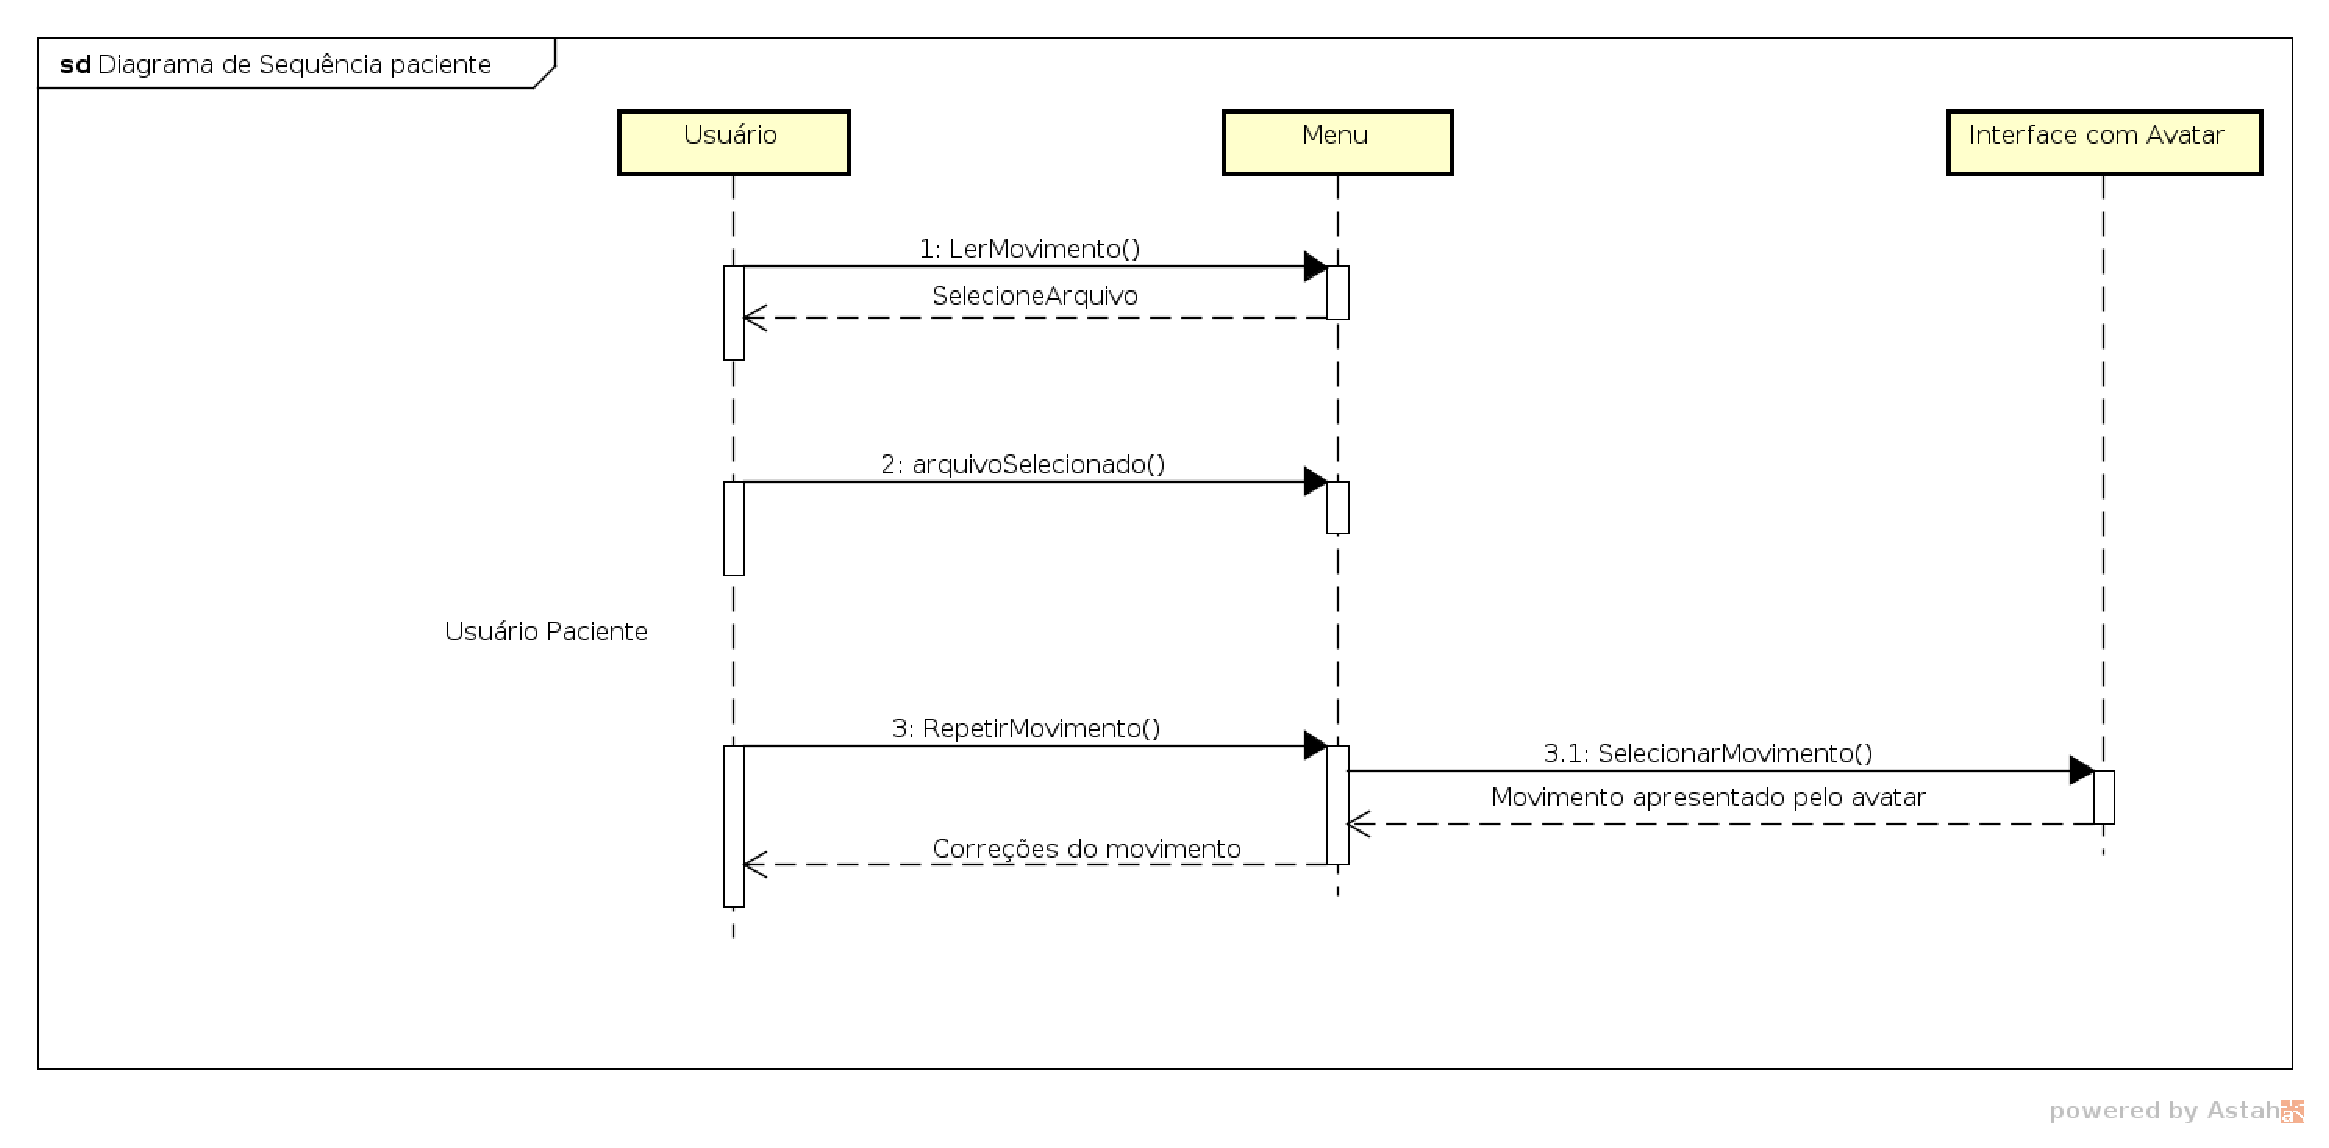
\includegraphics [keepaspectratio=true,scale=0.45]{figuras/diagramaPaciente.eps}

\caption{Diagrama de sequência referente ao uso do paciente}
\label{diagramaPaciente}
\end{figure}

  Para a criação desses artefatos foi utilizado a ferramenta Astah community que pode ser encontrada \href{http://astah.net/download#community}{aqui} gratuitamente.


\section{Fontes de Erro}\label{sol:fontesErro}
\section{Análise de viabilidade}\label{sol:viabilidade}
  Como
\subsection{Arquitetura}
